%%& -job-name=title_notes

\documentclass[10pt,xcolor=table,dvipsnames]{beamer}
% \documentclass[handout,10pt,xcolor=table,dvipsnames]{beamer}


\usepackage{handoutWithNotes}

\DeclareMathOperator\arctanh{arctanh}
\mode<presentation>
{
  %\usetheme[secheader]{Custom}
	\usetheme[secheader]{NTU}
  \setbeamercovered{invisible}
  % or whatever (possibly just delete it)
}
\setbeamertemplate{caption}{\raggedright\insertcaption\par}

\usepackage{pgfpages}
\usepackage{booktabs}
\usepackage{multirow}
\usepackage{graphicx}
\usepackage{subfig}
%\usepackage[labelformat=simple]{subfig}

\newcommand{\VI}{\mathrm{VI}}
%\setbeameroption{show notes on second screen}
\newcommand{\tb}[1]{\textbf{#1}}



\usepackage[T1]{fontenc}
\usepackage{lmodern}
\usepackage{amsmath,amssymb,amsfonts,mathrsfs,bm}% Typical maths resource packages
\usepackage{mathtools}
\usepackage{amsthm}
\usepackage{array}
\usepackage{graphicx}
\usepackage{epstopdf}
\DeclareGraphicsExtensions{.eps,.png,.jpg,.pdf}

%\usepackage[tight, footnotesize]{subfigure}
\usepackage{url}
\usepackage{algorithm,algorithmic}
\usepackage{color}
\usepackage[normalem]{ulem}
\usepackage{multirow}
\usepackage{array}
\newcolumntype{L}[1]{>{\raggedright\let\newline\\\arraybackslash\hspace{0pt}}m{#1}}
\newcolumntype{C}[1]{>{\centering\let\newline\\\arraybackslash\hspace{0pt}}m{#1}}
\newcolumntype{R}[1]{>{\raggedleft\let\newline\\\arraybackslash\hspace{0pt}}m{#1}}
\usepackage{xparse}

%\usepackage[style=ieee,backend=bibtex]{biblatex}
%\newcommand{\ifprefchar}{\ifpunctmark{'}} %restore functionality with BibTeX as a work-around
\usepackage[backend=biber, citestyle=numeric, bibstyle=ieee, sorting=none]{biblatex}


%\makeatletter%
%\@addtoreset{footnote}{page}
%\long\def\@makefnmark{%
%\hbox {{\normalfont [\@thefnmark]}}}%
%\makeatother

%\renewcommand{\thefootnote}{\ifcase\value{footnote}\or$\dagger$\or$\ddagger$\or$*$\or$\circ$\or$\diamond$\or$+$\or$\square$\or$\bot$\fi}
%\newcommand<>{\ftcite}[1]{
	%\footnote#2{\fullcite{#1}}
%}


\setbeamertemplate{bibliography item}{\insertbiblabel}

\makeatletter
\newcommand*{\mkblankfootnote}[1]{%
  \begingroup
    \renewcommand\thefootnote{}%
    \footnotetext{\bibfootnotewrapper{#1}}%
  \endgroup
}

\newcommand*{\mkbibsupercite}[1]{%
  \def\cbx@savedcites{\cbx@footfullcite}%
  \mkbibbrackets{#1}%
  \cbx@savedcites}

\DeclareCiteCommand{\supercite}[\mkbibsupercite]
  {\gdef\cbx@savedkeys{}}
  {\usebibmacro{citeindex}%
   \usebibmacro{cite}%
     {}%
   \xappto\cbx@savedkeys{\thefield{entrykey},}}
  {\supercitedelim}
  {\protected@xappto\cbx@savedcites{%
     [\thefield{prenote}][\thefield{postnote}]{\cbx@savedkeys}}}

\DeclareCiteCommand{\cbx@footfullcite}
  {}
  {\mkblankfootnote{%
     \printtext[labelnumberwidth]{%
       \usebibmacro{cite}%
     }%
   \setunit{\addspace}%
   \usedriver
     {\DeclareNameAlias{sortname}{default}}
     {\thefield{entrytype}}}}
  {}
  {}
\makeatother
\newcommand<>{\ftcite}[1]{\only#2{\supercite{#1}}}

\newcommand{\backupbegin}{
   \newcounter{framenumberappendix}
   \setcounter{framenumberappendix}{\value{framenumber}}
}
\newcommand{\backupend}{
   \addtocounter{framenumberappendix}{-\value{framenumber}}
   \addtocounter{framenumber}{\value{framenumberappendix}} 
}

\newcommand\Fontvi{\fontsize{10}{11}\selectfont}
\newcommand\Fontvismall{\fontsize{9}{9}\selectfont}
\renewcommand\arraystretch{1.5}% (MyValue=1.0 is for standard spacing)


%%%%%%%%%%%%%%%%%%%%%%%%%%%%%%%%%%%%%%%%

%Theorem declarations

% for use in main body
\newtheorem*{Proposition}{Proposition}
\newtheorem*{Remark}{Remark}
\newtheorem*{Assumption}{Assumption}
\newtheorem*{Exercise}{Exercise}

% Remarks
\theoremstyle{remark}
\newtheorem*{Rem}{Remark}

\newenvironment{remarks}{
	\begin{list}{\textit{Remark} \arabic{Rem}:~}{
    \setcounter{enumi}{\value{Rem}}
    \usecounter{Rem}
    \setcounter{Rem}{\value{enumi}}
    \setlength\labelwidth{0in}
    \setlength\labelsep{0in}
    \setlength\leftmargin{0in}
    \setlength\listparindent{0in}
    \setlength\itemindent{15pt}
		}
}{
	\end{list}
}

% Special Headings
%\newtheorem*{Prop1}{Proposition 1} %needs amsthm

%\newtheoremstyle{nonum}{}{}{\itshape}{}{\bfseries}{.}{ }{#1 (\mdseries #3)}
%\theoremstyle{nonum}
%\newtheorem{Example**}{Example 1}

\newcommand{\EndExample}{{$\square$}}
%\renewcommand{\QED}{\QEDopen} % changes end of proof box to open box.



%Number sets
\newcommand{\Real}{\mathbb{R}}
\newcommand{\Nat}{\mathbb{N}}
\newcommand{\Rat}{\mathbb{Q}}
\newcommand{\Complex}{\mathbb{C}}

% imaginary number i
\newcommand{\iu}{\mathfrak{i}\mkern1mu}


% Calligraphic stuff
\newcommand{\calA}{\mathcal{A}}
\newcommand{\calB}{\mathcal{B}}
\newcommand{\calC}{\mathcal{C}}
\newcommand{\calD}{\mathcal{D}}
\newcommand{\calE}{\mathcal{E}}
\newcommand{\calF}{\mathcal{F}}
\newcommand{\calG}{\mathcal{G}}
\newcommand{\calH}{\mathcal{H}}
\newcommand{\calI}{\mathcal{I}}
\newcommand{\calJ}{\mathcal{J}}
\newcommand{\calK}{\mathcal{K}}
\newcommand{\calL}{\mathcal{L}}
\newcommand{\calM}{\mathcal{M}}
\newcommand{\calN}{\mathcal{N}}
\newcommand{\calO}{\mathcal{O}}
\newcommand{\calP}{\mathcal{P}}
\newcommand{\calQ}{\mathcal{Q}}
\newcommand{\calR}{\mathcal{R}}
\newcommand{\calS}{\mathcal{S}}
\newcommand{\calT}{\mathcal{T}}
\newcommand{\calU}{\mathcal{U}}
\newcommand{\calV}{\mathcal{V}}
\newcommand{\calW}{\mathcal{W}}
\newcommand{\calX}{\mathcal{X}}
\newcommand{\calY}{\mathcal{Y}}
\newcommand{\calZ}{\mathcal{Z}}


% Boldface stuff
\newcommand{\ba}{\mathbf{a}}
\newcommand{\bA}{\mathbf{A}}
\newcommand{\bb}{\mathbf{b}}
\newcommand{\bB}{\mathbf{B}}
\newcommand{\bc}{\mathbf{c}}
\newcommand{\bC}{\mathbf{C}}
\newcommand{\bd}{\mathbf{d}}
\newcommand{\bD}{\mathbf{D}}
\newcommand{\be}{\mathbf{e}}
\newcommand{\bE}{\mathbf{E}}
\newcommand{\boldf}{\mathbf{f}}
\newcommand{\bF}{\mathbf{F}}
\newcommand{\bg}{\mathbf{g}}
\newcommand{\bG}{\mathbf{G}}
\newcommand{\bh}{\mathbf{h}}
\newcommand{\bH}{\mathbf{H}}
\newcommand{\bi}{\mathbf{i}}
\newcommand{\bI}{\mathbf{I}}
\newcommand{\bj}{\mathbf{j}}
\newcommand{\bJ}{\mathbf{J}}
\newcommand{\bk}{\mathbf{k}}
\newcommand{\bK}{\mathbf{K}}
\newcommand{\bl}{\mathbf{l}}
\newcommand{\bL}{\mathbf{L}}
\newcommand{\boldm}{\mathbf{m}}
\newcommand{\bM}{\mathbf{M}}
\newcommand{\bn}{\mathbf{n}}
\newcommand{\bN}{\mathbf{N}}
\newcommand{\bo}{\mathbf{o}}
\newcommand{\bO}{\mathbf{O}}
\newcommand{\bp}{\mathbf{p}}
\newcommand{\bP}{\mathbf{P}}
\newcommand{\bq}{\mathbf{q}}
\newcommand{\bQ}{\mathbf{Q}}
\newcommand{\br}{\mathbf{r}}
\newcommand{\bR}{\mathbf{R}}
\newcommand{\bs}{\mathbf{s}}
\newcommand{\bS}{\mathbf{S}}
\newcommand{\bt}{\mathbf{t}}
\newcommand{\bT}{\mathbf{T}}
\newcommand{\bu}{\mathbf{u}}
\newcommand{\bU}{\mathbf{U}}
\newcommand{\bv}{\mathbf{v}}
\newcommand{\bV}{\mathbf{V}}
\newcommand{\bw}{\mathbf{w}}
\newcommand{\bW}{\mathbf{W}}
\newcommand{\bx}{\mathbf{x}}
\newcommand{\bX}{\mathbf{X}}
\newcommand{\by}{\mathbf{y}}
\newcommand{\bY}{\mathbf{Y}}
\newcommand{\bz}{\mathbf{z}}
\newcommand{\bZ}{\mathbf{Z}}


% Numbers bb font
\newcommand{\bbA}{\mathbb{A}}
\newcommand{\bbB}{\mathbb{B}}
\newcommand{\bbC}{\mathbb{C}}
\newcommand{\bbD}{\mathbb{D}}
\newcommand{\bbE}{\mathbb{E}}
\newcommand{\bbF}{\mathbb{F}}
\newcommand{\bbG}{\mathbb{G}}
\newcommand{\bbH}{\mathbb{H}}
\newcommand{\bbI}{\mathbb{I}}
\newcommand{\bbJ}{\mathbb{J}}
\newcommand{\bbK}{\mathbb{K}}
\newcommand{\bbL}{\mathbb{L}}
\newcommand{\bbM}{\mathbb{M}}
\newcommand{\bbN}{\mathbb{N}}
\newcommand{\bbO}{\mathbb{O}}
\newcommand{\bbP}{\mathbb{P}}
\newcommand{\bbQ}{\mathbb{Q}}
\newcommand{\bbR}{\mathbb{R}}
\newcommand{\bbS}{\mathbb{S}}
\newcommand{\bbT}{\mathbb{T}}
\newcommand{\bbU}{\mathbb{U}}
\newcommand{\bbV}{\mathbb{V}}
\newcommand{\bbW}{\mathbb{W}}
\newcommand{\bbX}{\mathbb{X}}
\newcommand{\bbY}{\mathbb{Y}}
\newcommand{\bbZ}{\mathbb{Z}}


% Mathfrak font
\newcommand{\frakA}{\mathfrak{A}}
\newcommand{\frakB}{\mathfrak{B}}
\newcommand{\frakC}{\mathfrak{C}}
\newcommand{\frakD}{\mathfrak{D}}
\newcommand{\frakE}{\mathfrak{E}}
\newcommand{\frakF}{\mathfrak{F}}
\newcommand{\frakG}{\mathfrak{G}}
\newcommand{\frakH}{\mathfrak{H}}
\newcommand{\frakI}{\mathfrak{I}}
\newcommand{\frakJ}{\mathfrak{J}}
\newcommand{\frakK}{\mathfrak{K}}
\newcommand{\frakL}{\mathfrak{L}}
\newcommand{\frakM}{\mathfrak{M}}
\newcommand{\frakN}{\mathfrak{N}}
\newcommand{\frakO}{\mathfrak{O}}
\newcommand{\frakP}{\mathfrak{P}}
\newcommand{\frakQ}{\mathfrak{Q}}
\newcommand{\frakR}{\mathfrak{R}}
\newcommand{\frakS}{\mathfrak{S}}
\newcommand{\frakT}{\mathfrak{T}}
\newcommand{\frakU}{\mathfrak{U}}
\newcommand{\frakV}{\mathfrak{V}}
\newcommand{\frakW}{\mathfrak{W}}
\newcommand{\frakX}{\mathfrak{X}}
\newcommand{\frakY}{\mathfrak{Y}}
\newcommand{\frakZ}{\mathfrak{Z}}


% Mathscr
\newcommand{\scA}{\mathscr{A}}
\newcommand{\scB}{\mathscr{B}}
\newcommand{\scC}{\mathscr{C}}
\newcommand{\scD}{\mathscr{D}}
\newcommand{\scE}{\mathscr{E}}
\newcommand{\scF}{\mathscr{F}}
\newcommand{\scG}{\mathscr{G}}
\newcommand{\scH}{\mathscr{H}}
\newcommand{\scI}{\mathscr{I}}
\newcommand{\scJ}{\mathscr{J}}
\newcommand{\scK}{\mathscr{K}}
\newcommand{\scL}{\mathscr{L}}
\newcommand{\scM}{\mathscr{M}}
\newcommand{\scN}{\mathscr{N}}
\newcommand{\scO}{\mathscr{O}}
\newcommand{\scP}{\mathscr{P}}
\newcommand{\scQ}{\mathscr{Q}}
\newcommand{\scR}{\mathscr{R}}
\newcommand{\scS}{\mathscr{S}}
\newcommand{\scT}{\mathscr{T}}
\newcommand{\scU}{\mathscr{U}}
\newcommand{\scV}{\mathscr{V}}
\newcommand{\scW}{\mathscr{W}}
\newcommand{\scX}{\mathscr{X}}
\newcommand{\scY}{\mathscr{Y}}
\newcommand{\scZ}{\mathscr{Z}}


% define some useful uppercase Greek letters in regular and bold sf
\DeclareSymbolFont{bsfletters}{OT1}{cmss}{bx}{n}
\DeclareSymbolFont{ssfletters}{OT1}{cmss}{m}{n}
\DeclareMathSymbol{\bsfGamma}{0}{bsfletters}{'000}
\DeclareMathSymbol{\ssfGamma}{0}{ssfletters}{'000}
\DeclareMathSymbol{\bsfDelta}{0}{bsfletters}{'001}
\DeclareMathSymbol{\ssfDelta}{0}{ssfletters}{'001}
\DeclareMathSymbol{\bsfTheta}{0}{bsfletters}{'002}
\DeclareMathSymbol{\ssfTheta}{0}{ssfletters}{'002}
\DeclareMathSymbol{\bsfLambda}{0}{bsfletters}{'003}
\DeclareMathSymbol{\ssfLambda}{0}{ssfletters}{'003}
\DeclareMathSymbol{\bsfXi}{0}{bsfletters}{'004}
\DeclareMathSymbol{\ssfXi}{0}{ssfletters}{'004}
\DeclareMathSymbol{\bsfPi}{0}{bsfletters}{'005}
\DeclareMathSymbol{\ssfPi}{0}{ssfletters}{'005}
\DeclareMathSymbol{\bsfSigma}{0}{bsfletters}{'006}
\DeclareMathSymbol{\ssfSigma}{0}{ssfletters}{'006}
\DeclareMathSymbol{\bsfUpsilon}{0}{bsfletters}{'007}
\DeclareMathSymbol{\ssfUpsilon}{0}{ssfletters}{'007}
\DeclareMathSymbol{\bsfPhi}{0}{bsfletters}{'010}
\DeclareMathSymbol{\ssfPhi}{0}{ssfletters}{'010}
\DeclareMathSymbol{\bsfPsi}{0}{bsfletters}{'011}
\DeclareMathSymbol{\ssfPsi}{0}{ssfletters}{'011}
\DeclareMathSymbol{\bsfOmega}{0}{bsfletters}{'012}
\DeclareMathSymbol{\ssfOmega}{0}{ssfletters}{'012}


% Bold greek
\newcommand{\balpha}{\bm{\alpha}}
\newcommand{\bbeta}{\bm{\beta}}
\newcommand{\bgamma}{\bm{\gamma}}
\newcommand{\bdelta}{\bm{\delta}}
\newcommand{\btheta}{\bm{\theta}}
\newcommand{\bmu}{\bm{\mu}}
\newcommand{\bnu}{\bm{\nu}}
\newcommand{\btau}{\bm{\tau}}
\newcommand{\bpi}{\bm{\pi}}
\newcommand{\bepsilon}{\bm{\epsilon}}
\newcommand{\veps}{\varepsilon}
\newcommand{\bvarepsilon}{\bm{\varepsilon}}
\newcommand{\bsigma}{\bm{\sigma}}
\newcommand{\bvarsigma}{\bm{\varsigma}}
\newcommand{\bzeta}{\bm{\zeta}}
\newcommand{\bmeta}{\bm{\eta}}
\newcommand{\bkappa}{\bm{\kappa}}
\newcommand{\bchi}{\bm{\chi}}
\newcommand{\bphi}{\bm{\phi}}
\newcommand{\bpsi}{\bm{\psi}}
\newcommand{\bomega}{\bm{\omega}}
\newcommand{\bxi}{\bm{\xi}}
\newcommand{\blambda}{\bm{\lambda}}
\newcommand{\brho}{\bm{\rho}}

\newcommand{\bGamma}{\bm{\Gamma}}
\newcommand{\bLambda}{\bm{\Lambda}}
\newcommand{\bSigma	}{\bm{\Sigma}}
\newcommand{\bPsi}{\bm{\Psi}}
\newcommand{\bDelta}{\bm{\Delta}}
\newcommand{\bXi}{\bm{\Xi}}
\newcommand{\bUpsilon}{\bm{\Upsilon}}
\newcommand{\bOmega}{\bm{\Omega}}
\newcommand{\bPhi}{\bm{\Phi}}
\newcommand{\bPi}{\bm{\Pi}}
\newcommand{\bTheta}{\bm{\Theta}}

\newcommand{\talpha}{\widetilde{\alpha}}
\newcommand{\tbeta}{\widetilde{\beta}}
\newcommand{\tgamma}{\widetilde{\gamma}}
\newcommand{\tdelta}{\widetilde{\delta}}
\newcommand{\ttheta}{\widetilde{\theta}}
\newcommand{\tmu}{\widetilde{\mu}}
\newcommand{\tnu}{\widetilde{\nu}}
\newcommand{\ttau}{\widetilde{\tau}}
\newcommand{\tpi}{\widetilde{\pi}}
\newcommand{\tepsilon}{\widetilde{\epsilon}}
\newcommand{\tvarepsilon}{\widetilde{\varepsilon}}
\newcommand{\tsigma}{\widetilde{\sigma}}
\newcommand{\tzeta}{\widetilde{\zeta}}
\newcommand{\tmeta}{\widetilde{\eta}}
\newcommand{\tkappa}{\widetilde{\kappa}}
\newcommand{\tchi}{\widetilde{\chi}}
\newcommand{\tphi}{\widetilde{\phi}}
\newcommand{\tpsi}{\widetilde{\psi}}
\newcommand{\tomega}{\widetilde{\omega}}
\newcommand{\txi}{\widetilde{\xi}}
\newcommand{\tlambda}{\widetilde{\lambda}}
\newcommand{\trho}{\widetilde{\rho}}

\newcommand{\tbAlpha}{\widetilde{\bAlpha}}
\newcommand{\tbBeta}{\widetilde{\bBeta}}
\newcommand{\tbGamma}{\widetilde{\bGamma}}
\newcommand{\tbDelta}{\widetilde{\bDelta}}
\newcommand{\tbTheta}{\widetilde{\bTheta}}
\newcommand{\tbPi}{\widetilde{\bPi}}
\newcommand{\tbSigma}{\widetilde{\bSigma}}
\newcommand{\tbPhi}{\widetilde{\bPhi}}
\newcommand{\tbPsi}{\widetilde{\bPsi}}
\newcommand{\tbOmega}{\widetilde{\bOmega}}
\newcommand{\tbXi}{\widetilde{\bXi}}
\newcommand{\tbLambda}{\widetilde{\bLambda}}

\newcommand{\halpha}{\widehat{\alpha}}
\newcommand{\hbeta}{\widehat{\beta}}
\newcommand{\hgamma}{\widehat{\gamma}}
\newcommand{\hdelta}{\widehat{\delta}}
\newcommand{\htheta}{\widehat{\theta}}
\newcommand{\hmu}{\widehat{\mu}}
\newcommand{\hnu}{\widehat{\nu}}
\newcommand{\htau}{\widehat{\tau}}
\newcommand{\hpi}{\widehat{\pi}}
\newcommand{\hepsilon}{\widehat{\epsilon}}
\newcommand{\hvarepsilon}{\widehat{\varepsilon}}
\newcommand{\hsigma}{\widehat{\sigma}}
\newcommand{\hzeta}{\widehat{\zeta}}
\newcommand{\hmeta}{\widehat{\eta}}
\newcommand{\hkappa}{\widehat{\kappa}}
\newcommand{\hchi}{\widehat{\chi}}
\newcommand{\hphi}{\widehat{\phi}}
\newcommand{\barbPhi}{\bar{\bPhi}}
\newcommand{\hpsi}{\widehat{\psi}}
\newcommand{\homega}{\widehat{\omega}}
\newcommand{\hxi}{\widehat{\xi}}
\newcommand{\hlambda}{\widehat{\lambda}}
\newcommand{\hrho}{\widehat{\rho}}


% stackrel
\newcommand{\convp}{\stackrel{\mathrm{p}}{\longrightarrow}}
\newcommand{\convas}{\stackrel{\mathrm{a.s.}}{\longrightarrow}}
\newcommand{\convd}{\stackrel{\mathrm{d}}{\longrightarrow}}
\newcommand{\convD}{\stackrel{\mathrm{D}}{\longrightarrow}}

\newcommand{\dotleq}{\stackrel{.}{\leq}}
\newcommand{\dotlt}{\stackrel{.}{<}}
\newcommand{\dotgeq}{\stackrel{.}{\geq}}
\newcommand{\dotgt}{\stackrel{.}{>}}
\newcommand{\dotdoteq}{\stackrel{\,..}{=}}

\newcommand{\eqa}[1]{\stackrel{#1}{=}}
\newcommand{\ed}{\eqa{\mathrm{d}}}
\newcommand{\lea}[1]{\stackrel{#1}{\le}}
\newcommand{\gea}[1]{\stackrel{#1}{\ge}}

%MathOperator
\DeclareMathOperator*{\argmax}{arg\,max}
\DeclareMathOperator*{\argmin}{arg\,min}
\DeclareMathOperator*{\argsup}{arg\,sup}
\DeclareMathOperator*{\arginf}{arg\,inf}
\DeclareMathOperator{\minimize}{minimize}
\DeclareMathOperator{\maximize}{maximize}
\DeclareMathOperator{\st}{s.t.}
%\DeclareMathOperator{\st}{subject\,\,to}
\DeclareMathOperator{\as}{a.s.}
\DeclareMathOperator{\diag}{diag}
\DeclareMathOperator{\cum}{cum}
\DeclareMathOperator{\sgn}{sgn}
\DeclareMathOperator{\tr}{tr}
\DeclareMathOperator{\Tr}{Tr}
\DeclareMathOperator{\spn}{span}
\DeclareMathOperator{\supp}{supp}
\DeclareMathOperator{\adj}{adj}
\DeclareMathOperator{\var}{var}
\DeclareMathOperator{\Vol}{Vol}
\DeclareMathOperator{\cov}{cov}
\DeclareMathOperator{\corr}{corr}
\DeclareMathOperator{\sech}{sech}
\DeclareMathOperator{\sinc}{sinc}
\DeclareMathOperator{\rank}{rank}
\DeclareMathOperator{\poly}{poly}
\DeclareMathOperator{\vect}{vec}
\DeclareMathOperator{\conv}{conv}
\DeclareMathOperator*{\lms}{l.i.m.\,}
\DeclareMathOperator*{\esssup}{ess\,sup}
\DeclareMathOperator*{\essinf}{ess\,inf}
\DeclareMathOperator{\sign}{sign}
\DeclareMathOperator{\eig}{eig}

%Paired delimiters
\DeclarePairedDelimiter\abs{\lvert}{\rvert}
\DeclarePairedDelimiter\parens{(}{)}
\DeclarePairedDelimiter\brk{[}{]}
\DeclarePairedDelimiter\braces{\{}{\}}



\newcommand{\qednew}{\nobreak \ifvmode \relax \else
      \ifdim\lastskip<1.5em \hskip-\lastskip
      \hskip1.5em plus0em minus0.5em \fi \nobreak
      \vrule height0.75em width0.5em depth0.25em\fi}

\newcommand{\nn}{\nonumber\\}


\newcommand{\T}{^{\intercal}}% transpose notation
\newcommand{\setcomp}{^{\mathsf{c}}} %set complement
\newcommand{\ud}{\mathrm{d}}
\newcommand{\Id}{\mathrm{Id}}
\newcommand{\Bigmid}{{\ \Big| \ }}
\newcommand{\bzero}{\mathbf{0}}
\newcommand{\bone}{\mathbf{1}}

%Combined Aliases
\newcommand{\indicator}[1]{{\bf 1}_{\braces*{#1}}}
\newcommand{\indicatore}[1]{{\bf 1}_{#1}}
\newcommand{\indicate}[1]{{\bf 1}\braces*{#1}}
\newcommand{\ofrac}[1]{{\frac{1}{#1}}}
\newcommand{\ddfrac}[2]{{\frac{\ud {#1}}{\ud {#2}}}}
\newcommand{\ppfrac}[2]{\frac{\partial {#1}}{\partial {#2}}}
\newcommand{\tc}[1]{^{(#1)}}
\newcommand{\ceil}[1]{\left\lceil{#1}\right\rceil}
\newcommand{\floor}[1]{\left\lfloor{#1}\right\rfloor}
\newcommand{\ip}[2]{{\left\langle{#1},\, {#2}\right\rangle}}
\newcommand{\norm}[1]{{\left\lVert{#1}\right\rVert}}
\newcommand{\trace}[1]{{\Tr\left( #1 \right)}}
\newcommand{\col}[1]{\operatorname{col}\left\{{#1}\right\}}% column vector
\newcommand{\row}[1]{\operatorname{row}\left\{{#1}\right\}}% row vector
\newcommand{\erf}[1]{\operatorname{erf}\parens*{#1}}
\newcommand{\erfc}[1]{\operatorname{erfc}\parens*{#1}}

\newcommand{\KLD}[2]{{D({#1}\, ||\, {#2})}}
\newcommand{\Lh}[1]{\ell_{#1}}
\newcommand{\LLh}[1]{\log{\Lh{#1}}}
\newcommand{\cond}[2]{\left. {#1}\, \middle| \, {#2} \right.}

\newcommand{\ml}[1]{\begin{multlined}#1\end{multlined}}


\DeclareDocumentCommand \ifcond {m m} {%
	{#1} %
	\IfValueT{#2}{\, \middle|\, {#2}}%
}

%\newcommand\argProtect[1]{\def\ProcessedArgument{{#1}}}
	
% Allows the use of 
% \P : \mathbb{P}
% \P(X) : \mathbb{P}\left({X}\right)
% \P_{p}(X) or \P{p}(X) : \mathbb{P}_{p}\left({X}\right)
% \P(X @| Y) or \P(X){Y} : \mathbb{P}\left({X}\, \middle| \, {Y}\right). 
% \P_{p}(X @| Y) or \P{p}(X){Y} : \mathbb{P}_{p}\left({X}\, \middle| \, {Y}\right)
% Caveats: Iterated expressions do not work well with \P(X|Y) notation
% \P(\P(X @| Y) c| Z) does not work, use \P({\P(X @| Y)} c| Z) or \P(\P(X){Y} @| Z)
% \P(\P(X @| Y)) does not work, use \P( {\P(X @| Y)} )
\DeclareDocumentCommand \P {e{_} g >{\SplitArgument{ 1 }{ @| }}d() g } {%
	\mathbb{P}%
	\IfValueTF{#1}{_{#1}}
		{\IfValueT{#2}{_{#2}}}%
	\IfValueT{#3}{\left(\ifcond#3}%
	\IfValueT{#4}{\, \middle|\, {#4}}%
	\IfValueT{#3}{\right)}%
}

% Allows the use of 
% \E : \mathbb{E}
% \E[X] : \mathbb{E}\left[{X}\right]
% \E_{p}[X] or \E{p}[X] : \mathbb{E}_{p}\left[{X}\right]
% \E[X @| Y] or \E[X]{Y} : \mathbb{E}\left[{X}\, \middle| \, {Y}\right]. 
% \E_{p}[X @| Y] or \E{p}[X]{Y} : \mathbb{E}_{p}\left[{X}\, \middle| \, {Y}\right]
% Caveats: Iterated expressions do not work well with \E[X|Y] notation
% \E[\E[X @| Y] c| Z] does not work, use \E[{\E[X c| Y]}|Z] or \E[\E[X]{Y}|Z]
% \E[\E[X @| Y]] does not work, use \E[ {\E[X @| Y]} ]
\DeclareDocumentCommand \E {e{_} g >{\SplitArgument{ 1 }{ @| }}o g } {%
	\mathbb{E}%
	\IfValueTF{#1}{_{#1}}
		{\IfValueT{#2}{_{#2}}}%
	\IfValueT{#3}{\left[\ifcond#3}%
	\IfValueT{#4}{\, \middle|\, {#4}}%
	\IfValueT{#3}{\right]}%
}


\def\independenT#1#2{\mathrel{\rlap{$#1#2$}\mkern5mu{#1#2}}}
\newcommand\independent{\protect\mathpalette{\protect\independenT}{\perp}}
\newcommand{\Bern}[1]{\mathrm{Bern}\left(#1\right)}
\newcommand{\Unif}[1]{\mathrm{Unif}\left(#1\right)}
\newcommand{\Dir}[1]{\mathrm{Dir}\left(#1\right)}
\newcommand{\Cat}[1]{\mathrm{Cat}\left(#1\right)}
\newcommand{\N}[2]{{\calN\left({#1},\: {#2}\right)}}
\newcommand{\Beta}[2]{{\calB e\left({#1},\: {#2}\right)}}



%colors
\definecolor{gray90}{gray}{0.9}

\newcommand<>{\red}[1]{{\color#2{red} #1}}
\newcommand<>{\blue}[1]{{{\color#2{blue} #1}}}
\newcommand<>{\green}[1]{{\color#2{green} #1}}
\newcommand<>{\gray}[1]{{\color#2{gray} #1}}

\newcommand<>{\brown}[1]{{\color#2{brown} #1}}
\newcommand<>{\magenta}[1]{{\color#2{magenta} #1}}
\newcommand<>{\orange}[1]{{\color#2{orange} #1}}
\newcommand<>{\teal}[1]{{\color#2{teal} #1}}

%figures
\newcommand{\figref}[1]{\figurename~\ref{#1}}
\renewcommand{\figurename}{Fig.}
\graphicspath{{./Figures/}} 
\pdfsuppresswarningpagegroup=1

\usepackage{tikz}
\usetikzlibrary{shapes.geometric, arrows}
%\bibliography{IEEEabrv,StringDefinitions,DecentDet,BibBooks,Tay,Social,Infection,IoT}
%\bibliography{IEEEabrv,StringDefinitions,Tay,refs}
%\addbibresource{IEEEabrv.bib}	
%\addbibresource{StringDefinitions.bib}	
%\addbibresource{adv_dnn.bib}	

%\bibliography{\BIBLDIR/IEEEabrv,\BIBLDIR/StringDefinitions,\BIBLDIR/Privacy,\BIBLDIR/machine_learning,\BIBLDIR/DecentDet,\BIBLDIR/Optimization,\BIBLDIR/IoT,\BIBLDIR/Books}
\def\BIBLDIR{./Bib}            % directory of code snippets
%\bibliography{IEEEabrv,StringDefinitions,DecentDet,BibBooks,Tay,Social,Infection,IoT}
%\bibliography{\BIBLDIR/IEEEabrv,\BIBLDIR/StringDefinitions,\BIBLDIR/adv_dnn}		
\bibliography{IEEEabrv,StringDefinitions,adv_dnn}
%\graphicspath{{./Figures}}
%\addmediapath{{./Videos/}}



\title[Uniform Convergence of Function Sequences/Series]
{Uniform Convergence of Function Sequences/Series}    % Enter your title between curly braces
\author[Kang Qiyu]{
    Kang Qiyu
}
\institute{
    Nanyang Technological University\\
    50 Nanyang Ave, Singapore 639798 \\
   kang0080@e.ntu.edu.sg\\
}
\date{Sep. 2023}                    % Enter the date or \today between curly braces

\AtBeginSection[] % Do nothing for \section*
{
\begin{frame}<beamer>
\frametitle{Outline}
\tableofcontents[currentsection]
\end{frame}
}

\setbeamertemplate{caption}{\raggedright\insertcaption\par}

\begin{document}



% Creates title page of slide show using above information
\begin{frame}
  \titlepage
\end{frame}

%\begin{frame}{Rest of this talk ...}
%\tableofcontents
%\end{frame}


%\section{Preliminaries}
\begin{frame}{Motivation}
\centering{Why do we care about function sequences/series?}
\end{frame}

\begin{frame}{Motivation}
\vspace{-0.3cm}
\begin{itemize} {\small 
\item Stone-Weierstras theorem: can we ``uniformly'' well approximate an arbitrary continuous function $f$ over an interval using  polynomial sequence $\{P_n\}$?
\begin{figure}[!htb]
\centering
% \vspace{-0.7cm}
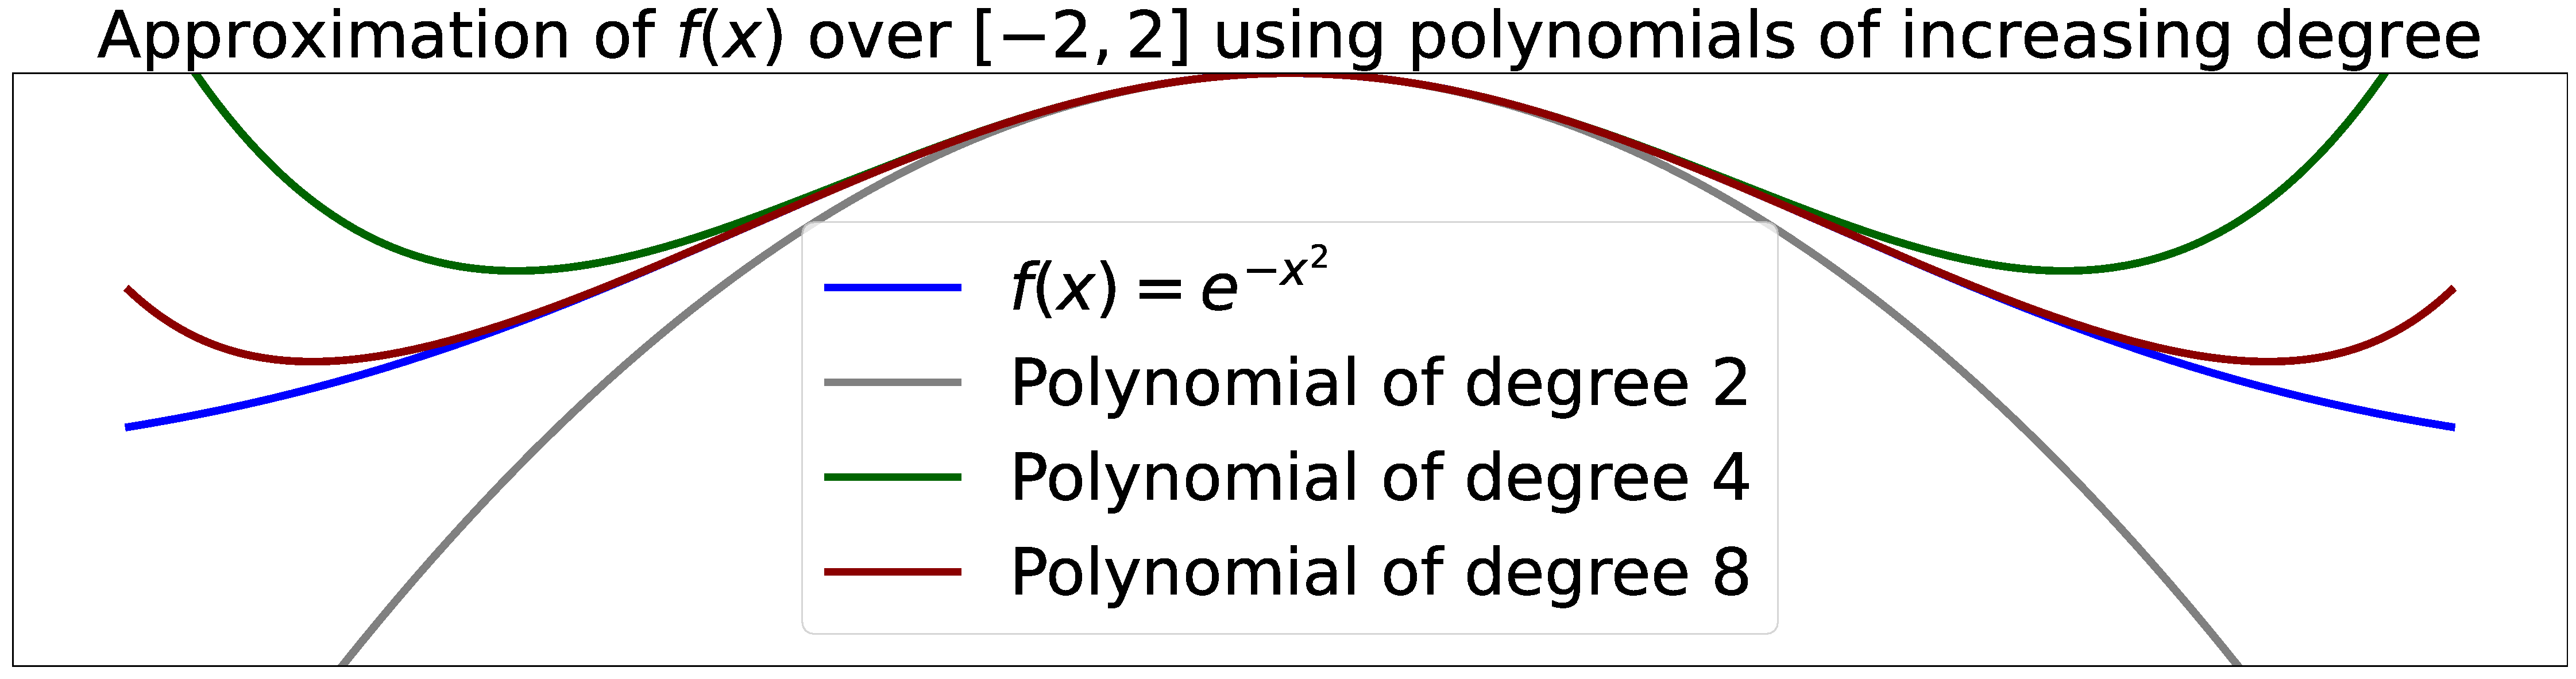
\includegraphics[width=0.5\textwidth]{Figures/swt.pdf}
\end{figure}
\pause
    \item neural network approximation capabilities as width $\rightarrow \infty$
\begin{figure}[!htb]
\centering
% \vspace{-0.7cm}
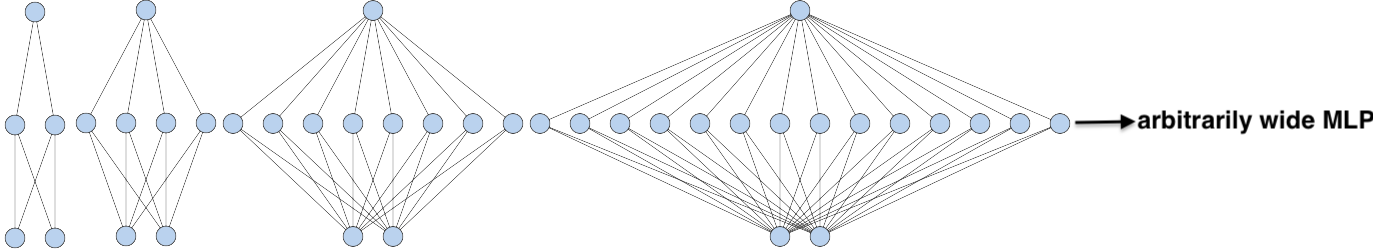
\includegraphics[width=0.9\textwidth]{Figures/uni_app.png}
% \label{fig:ecn}
\end{figure}
    \pause 
    \item sequential estimation/learning: {\small $Y_1(\omega)=f_1(X_1(\omega))$, $Y_2(\omega)=f_2(X_1(\omega),X_2(\omega))$, $\ldots$. How does the estimator $Y_n(\omega)$ behave? Can we get an arbitrarily good estimation of some unknown r.v. $Y(\omega)$ or parameter asymptotically?}
  \pause  \item numerical computation: E.g. numerically approximate incomplete gamma function 
$\gamma(a, x) \equiv \int_0^x \mathrm{e}^{-t} t^{a-1} \mathrm{~d} t \approx x^a \sum_{n=0}^{N} \frac{(-1)^n x^n}{(a+n) n !}.$
   \pause \item {\small network analysis (social, citation, collaboration): converge from increasing sized graphs to an asymptotic graphon (symmetric function $W:[0,1]^2 \mapsto[0,1]$)}}
\end{itemize}

\end{frame}

\section{Definitions of Function Convergence: Pointwise vs. Uniform}

\begin{frame}{Pointwise Convergence}
We confine our attention to complex- or real-valued functions.
\begin{Definition}[pointwise convergence]
    Suppose $\left\{f_n\right\}, n=1,2,3, \ldots$, is a sequence of functions defined on a set $E$, and suppose that the sequence of numbers $\left\{f_n(x)\right\}$ {converges for every $x \in E$}. We can then define a limit function $f$, by
\begin{align}
f(x)=\lim _{n \rightarrow \infty} f_n(x) \quad(x \in E) .
\end{align}
We say that ``$\left\{f_n\right\}$ converges to $f$ \blue{pointwise} on $E$''.
\end{Definition}
\tb{summary:} 
{\small $\left\{f_n\right\}$ converges to $f$ \blue{pointwise} on $E$
iff
$\lim _{n \rightarrow \infty} f_n(x)=f(x) \text{ for all } x \in E$.}
\pause
\begin{Remark}[Series]
    {\ Similarly, if $\sum f_n(x)$ converges for \blue{$x \in E$}, and if we define the limit function  as 
$f(x)=\sum_{n=1}^{\infty} f_n(x) \quad(x \in E).$
We say that ``$\sum f_n$ converges to $f$ \blue{pointwise} on $E$''.}
\end{Remark}
\end{frame}

\begin{frame}{Uniform Convergence}
Motivation:  The rate of convergence is ``uniform'' across the entire domain.
\begin{Definition}[uniform convergence]
   We say that a sequence of functions $\left\{f_n\right\}, n=1,2,3, \ldots$, \blue{converges uniformly} on $E$ to a function $f$ if for every $\varepsilon>0$ there is an integer $N$ such that $n \geq N$ implies
\begin{align}
\left|f_n(x)-f(x)\right| \leq \varepsilon
\end{align}
for all $x \in E$.
\end{Definition}
\tb{summary:} $\left\{f_n\right\}$ converges to $f$ \blue{uniformly} on $E$
iff $\forall \epsilon>0$, $\exists N$ s.t. $\sup_{x\in E} \left|f_n(x)-f(x)\right| \leq \varepsilon$ for all $n>N$.
\pause
\begin{Remark}[Series]
    {\ Similarly, the series $\sum f_n(x)$ converges \blue{uniformly} on $E$ if the sequence $\left\{s_n\right\}$ of partial sums defined by
$s_n(x)\coloneqq\sum_{i=1}^n f_i(x)$
converges \blue{uniformly} on $E$.}
\end{Remark}
\end{frame}

\begin{frame}{Comparison}
\begin{enumerate}
    \item \tb{pointwise convergence:} 
{
$\lim _{n \rightarrow \infty} f_n(x)=f(x) \text{ for all } x \in E$.}

\emph{\small \tb{equivalent $\varepsilon$-$\delta$ description:} for every $x>0$, and for every $\varepsilon \in E$, there is an integer \blue{$N(\varepsilon,x)$}, depending on $\varepsilon$ and on $x$, s.t. $\left|f_n(x)-f(x)\right| \leq \varepsilon$ holds if $n \geq N$.}
\pause
\item\tb{uniform convergence:} \emph{\small for every $\varepsilon>0$ there is an integer \blue{$N(\varepsilon)$}, depending only on $\varepsilon$, s.t.
$\left|f_n(x)-f(x)\right| \leq \varepsilon$ if $n\geq N$
for all $x \in E$.}
\end{enumerate}
\pause
\vspace{1cm}
\begin{itemize}
    \item \tb{Observation:} uniform convergence $\Rightarrow$ pointwise convergence.
   \pause \item \tb{Question:}  uniform convergence $\Leftarrow$ pointwise convergence?
\end{itemize}
\end{frame}

\begin{frame}{uniform convergence $\not\Leftarrow$ pointwise convergence}
\vspace{-0.3cm}
\begin{figure}[!htb]
\centering
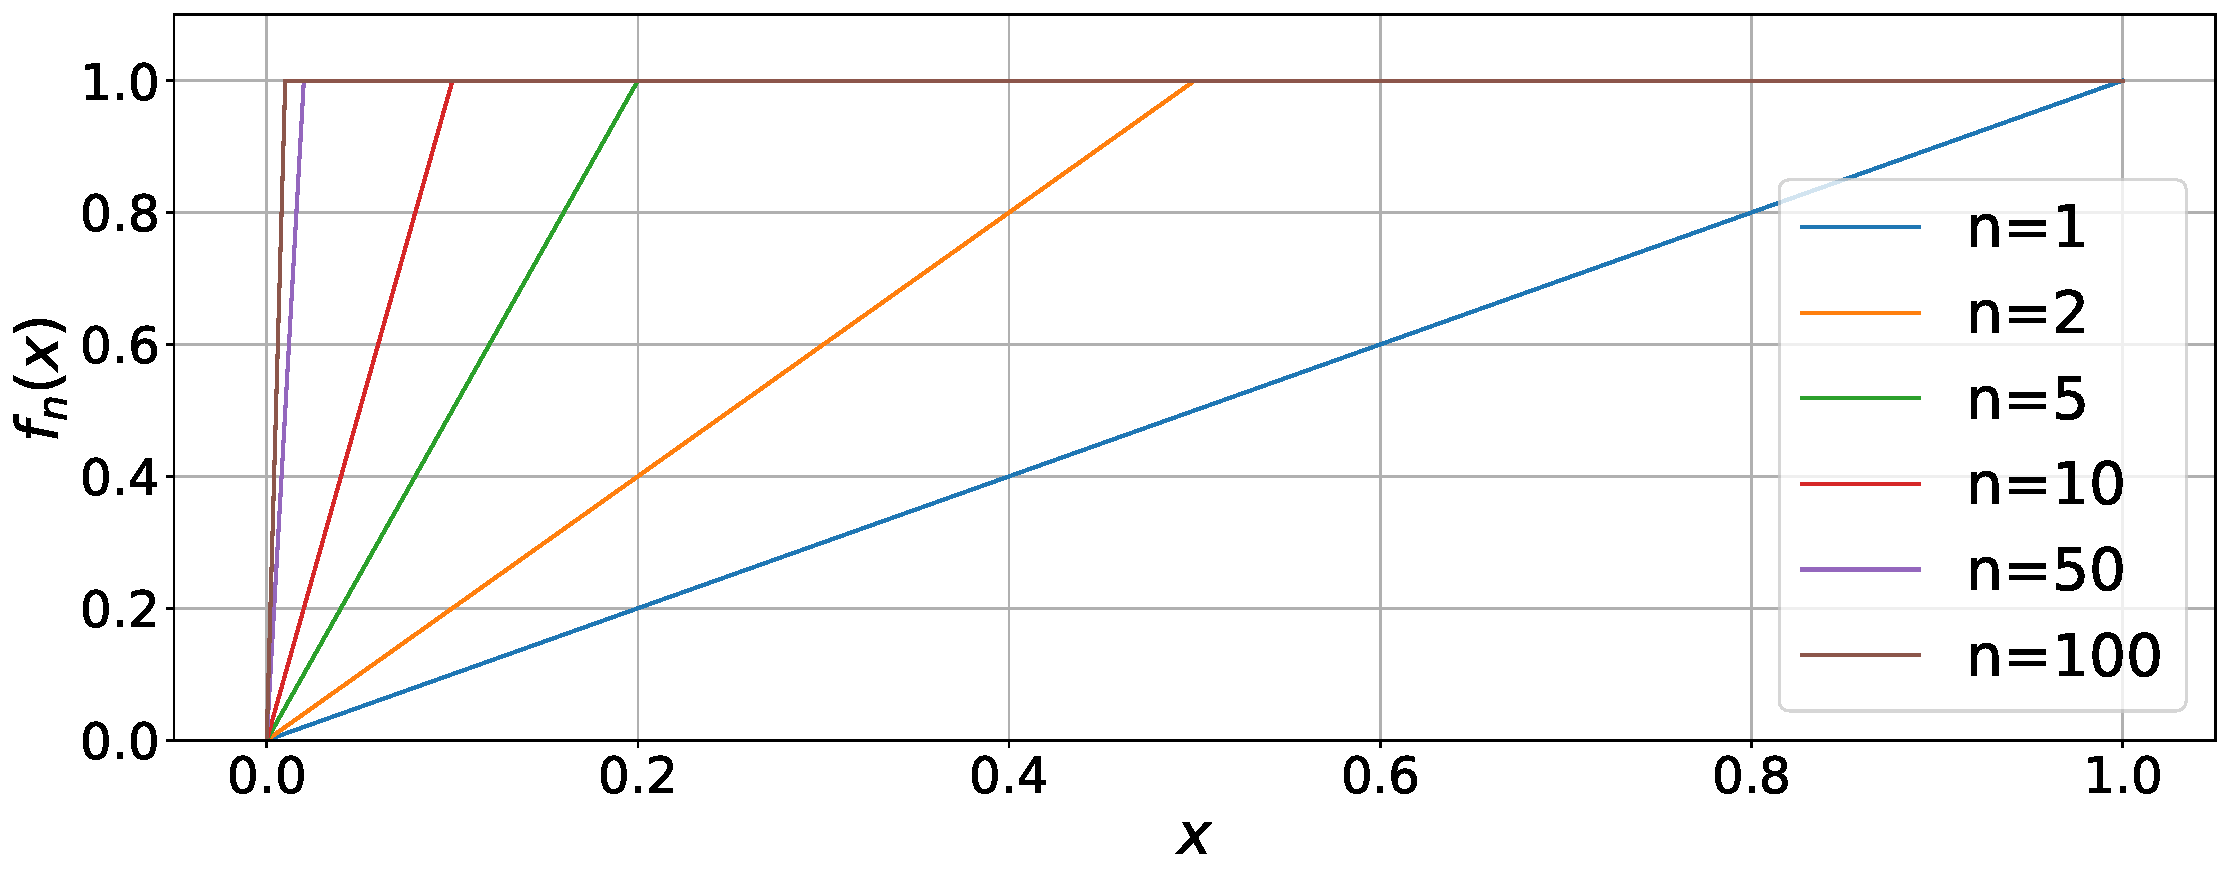
\includegraphics[width=0.6\textwidth]{Figures/exm1.pdf}
\end{figure}
\vspace{-0.3cm}
Consider $\{f_n(x)\}$ defined on the interval $[0, 1]$ by:
\begin{align*}
f_n(x)= \begin{cases}n x & \text { for } 0 \leq x \leq \frac{1}{n} \\ 1 & \text { for } \frac{1}{n}<x \leq 1\end{cases}
\end{align*}
\tb{pointwisely convergent} to 
\begin{align*}
f(x)= \begin{cases}0 & \text { for } x=0 \\ 1 & \text { for } 0<x \leq 1\end{cases}
\end{align*}
\tb{but \blue{not} uniformly:}
\begin{align*}
\left|f_n\left(\frac{1}{2n^2}\right)-f\left(\frac{1}{2n^2}\right)\right|=\left|n \cdot \frac{1}{2n^2}-1\right|=1-\frac{1}{2n}\ge \frac{1}{2}
\end{align*}
% No matter how large $n$ becomes, this difference remains 1.
\end{frame}

\section{Interchange of Limit Processes (e.g. \blue{continuous}, \blue{differentiable}, or integrable)}

\begin{frame}{Uniform Convergence and Continuity}
\begin{Theorem}[Interchanging Two Limits]
    Suppose $f_n \rightarrow f$ \blue{uniformly} on a set $E$ in a metric space. Let $x$ be a limit point of $E$, and assume the existence of $\lim _{t \rightarrow x} f_n(t)$ for all $n$, we have 
\begin{align*}
\lim _{t \rightarrow x} \lim _{n \rightarrow \infty} f_n(t)=\lim _{n \rightarrow \infty} \lim _{t \rightarrow x} f_n(t) .
\end{align*}
\end{Theorem}
\pause
\magenta{basic theorem $\Rightarrow$ theorems about continuous, differentiable. }

\pause
Proof Hint:
 Let a $\varepsilon$ be given.\\ 
Step 1: Define $A_n\coloneqq \lim _{t \rightarrow x} f_n(t)$. Uniform convergence $\Rightarrow$   $\exists N$ s.t.
$\left|f_n(t)-f_m(t)\right| \leq \varepsilon$ $\forall n, m \geq N, \blue{\forall t \in E}$.
It follows that
$\left|A_n-A_m\right| \leq \varepsilon$, a Cauchy sequence. So, it converges to a limit, denoted by $A$.

\pause
Step 2: $|f(t)-A| \leq\left|f(t)-f_n(t)\right|+\left|f_n(t)-A_n\right|+\left|A_n-A\right|$. Prove each item $< \varepsilon/3$ for large enough $n$ and for \( t \) sufficiently close to $x$. We therefore have $|f(t) - A| < \varepsilon$ when $t$ is sufficiently close to $x$.
\pause
\begin{Corollary}[Continuity Preserved under Uniform Convergence]
 If $\left\{f_n\right\}$ is a sequence of \blue{continuous} functions on $E$, and if $f_n \rightarrow f$ \blue{uniformly} on $E$, then $f$ is \blue{continuous} on $E$.
\end{Corollary}
\end{frame}


\begin{frame}{Example: pointwise convergence may lead to discontinuous}
Let
\begin{align*}
f_n(x)=\frac{x^2}{\left(1+x^2\right)^n} \quad(x \text { real } ; n=0,1,2, \ldots),
\end{align*}
and consider
\begin{align*}
f(x)=\sum_{n=0}^{\infty} f_n(x)=\sum_{n=0}^{\infty} \frac{x^2}{\left(1+x^2\right)^n} .
\end{align*}
Since $f_n(0)=0$, we have $f(0)=0$. For $x \neq 0$, the last series is a convergent geometric series with sum $1+x^2$. Hence
\begin{align*}
f(x)= \begin{cases}0 & (x=0), \\ 1+x^2 & (x \neq 0).\end{cases}
\end{align*}
{\small So, a \blue{pointwise convergent} series of continuous functions may have a \blue{discontinuous} sum.}    
\end{frame}

\begin{frame}{Uniform Convergence and Differentiation}
\begin{itemize}
    \item $f_n \rightarrow f$ uniformly $\Rightarrow$ the convergence of $f_n^{\prime} \rightarrow f^{\prime}$?  No! \\
    \pause
\emph{\small Example: 
\begin{align*}
f_n(x)=\frac{\sin n x}{\sqrt{n}} \quad(x \text { real, } n=1,2,3, \ldots),
\end{align*}
and
\begin{align*}
f(x)=\lim _{n \rightarrow \infty} f_n(x)=0 .
\end{align*}
Then $f^{\prime}(x)=0$, and
$f_n^{\prime}(x)=\sqrt{n} \cos n x,$
so that $\left\{f_n^{\prime}\right\}$ does not converge to $f^{\prime}$. For instance, $f_n^{\prime}(0)=\sqrt{n} \rightarrow+\infty$ as $n \rightarrow \infty$, whereas $f^{\prime}(0)=0$.}
\pause

So we need \brown{stronger hypotheses} to get $f_n^{\prime} \rightarrow f^{\prime}$!
\pause

\begin{Theorem}[Interchanging Limit and Differentiation]
    Suppose $\left\{f_n\right\}$ is a sequence of functions, differentiable on $[a, b]$ and such that $\left\{f_n\left(x_0\right)\right\}$ converges for some point $x_0$ on $[a, b]$. If \brown{$\left\{f_n^{\prime}\right\}$ converges uniformly} on $[a, b]$, then $\left\{f_n\right\}$ converges uniformly on $[a, b]$, to a function $f$, and
\begin{align*}
f^{\prime}(x)=\lim _{n \rightarrow \infty} f_n^{\prime}(x) \quad(a \leq x \leq b) .
\end{align*}
\end{Theorem}  

\end{itemize}
\end{frame}

\begin{frame}{Uniform Convergence and Differentiation}
\vspace{-0.3cm}
    Proof Hint: Let $\varepsilon>0$ be given.

 \tb{Step 1:} Prove $\left\{f_n\right\} \rightarrow f$ uniformly:

Uniform convergence of  $\left\{f_n^{\prime}\right\}$ leads to $\left|f_n^{\prime}(t)-f_m^{\prime}(t)\right|<\frac{\varepsilon}{2(b-a)} \quad(a \leq t \leq b)$ if $n, m \geq N_0$. 
Apply the mean value theorem to $f_n-f_m$ and get 
$\left|f_n(x)-f_m(x)-f_n(t)+f_m(t)\right| \leq \frac{|x-t| \varepsilon}{2(b-a)} \leq \frac{\varepsilon}{2}$.
Finally use 
$\left|f_n(x)-f_m(x)\right| \leq\left|f_n(x)-f_m(x)-f_n\left(x_0\right)+f_m\left(x_0\right)\right|+\left|f_n\left(x_0\right)-f_m\left(x_0\right)\right|<\varepsilon$ when $n,m>N_1$ for all $x$.

\vspace{0.3cm}
 \pause
\tb{Step 2:} Prove $\left\{\phi_n\right\} \rightarrow \phi(t)$ uniformly:
Fix a $x$ and define
\begin{align*}
\phi_n(t)=\frac{f_n(t)-f_n(x)}{t-x}, \quad \phi(t)=\frac{f(t)-f(x)}{t-x}
\end{align*}
for $a \leq t \leq b, t \neq x$.
\vspace{0.3cm}
 \pause
 
\tb{Step 3:} Interchanging  limits:
Since $\left\{f_n\right\}$ converges to $f$, it follows that
\begin{align*}
\lim _{n \rightarrow \infty} \phi_n(t)=\phi(t)
\end{align*}
uniformly for $a \leq t \leq b, t \neq x$.
Theorem (Interchanging Two Limits) show that
\begin{align*}
\lim _{t \rightarrow x} \phi(t)=\lim _{n \rightarrow \infty} f_n^{\prime}(x) ;
\end{align*}
\end{frame} 

\begin{frame}{Analytic Functions/Power Series}
\vspace{-0.3cm}
\begin{Lemma}[Uniform Convergence Test for Series]
  {\small  Suppose $\left\{f_n\right\}$ is a sequence of functions defined on $E$, and suppose
\begin{align*}
\left|f_n(x)\right| \leq M_n \quad(x \in E, n=1,2,3, \ldots) .
\end{align*}
Then $\sum f_n$ \blue{converges uniformly} on $E$ if $\sum M_n$ converges.}
\end{Lemma}
\pause
\vspace{-0.3cm}
\begin{Theorem}
{\small   Suppose the real-valued series
$\sum_{n=0}^{\infty} c_n x^n$
converges for $|x|<R$, and define
\begin{align}
f(x)=\sum_{n=0}^{\infty} c_n x^n \quad(|x|<R) .
\end{align}
Then the series converges \blue{uniformly} on $[-R+\varepsilon, R-\varepsilon]$, no matter which $\varepsilon>0$ is chosen. The function $f$ is continuous and differentiable in $(-R, R)$, and
% \vspace{-0.3cm}
\begin{align}
f^{\prime}(x)=\sum_{n=1}^{\infty} n c_n x^{n-1} \quad(|x|<R) .
\end{align} 
}
\end{Theorem}
{\small Proof Hint: Use the above Lemma and ``Interchanging Limit and Differentiation''.}

% Proof Let $\varepsilon>0$ be given. For $|x| \leq R-\varepsilon$, we have
% \begin{align*}
% \left|c_n x^n\right| \leq\left|c_n(R-\varepsilon)^n\right|
% \end{align*}
% and since
% \begin{align*}
% \sum c_n(R-\varepsilon)^n
% \end{align*}
% converges absolutely (every power series converges absolutely in the interior of its interval of convergence, by the root test), Theorem 7.10 shows the uniform convergence of (3) on $[-R+\varepsilon, R-\varepsilon]$.
% Since $\sqrt[n]{n} \rightarrow 1$ as $n \rightarrow \infty$, we have
% \begin{align*}
% \limsup _{n \rightarrow \infty} \sqrt[n]{n\left|c_n\right|}=\limsup _{n \rightarrow \infty} \sqrt[n]{\left|c_n\right|}
% \end{align*}
% so that the series (4) and (5) have the same interval of convergence.
% Since (5) is a power series, it converges uniformly in $[-R+\varepsilon$, $R-\varepsilon$ ], for every $\varepsilon>0$, and we can apply Theorem 7.17 (for series instead of sequences). It follows that (5) holds if $|x| \leq R-\varepsilon$.

% But, given any $x$ such that $|x|<R$, we can find an $\varepsilon>0$ such that $|x|<R-\varepsilon$. This shows that (5) holds for $|x|<R$.
% Continuity of $f$ follows from the existence of $f^{\prime}$ (Theorem 5.2).
\end{frame}

\begin{frame}{Post-Course Tasks and Recommended Readings}
    \begin{itemize}
        \item \blue{Self-write the complete proofs of discussed theorems.
        \item Complete all assigned homework.}
        \item Delve into Convergence Types: \( L_1 \) convergence, almost surely convergence, pointwise convergence, and uniform convergence.
        \item Investigate the Approximation Capabilities of Neural Networks [1].
        \item Explore the intricacies of Sequential Estimation [2].
        \item Explore Neural Ordinary Differential Equations [3] and the associated existence and uniqueness of solutions: Picard–Lindelöf theorem [4] where the function sequence and uniform convergence are used in the proof.
    \end{itemize}
\end{frame}


\begin{frame}{References}
    \begin{itemize}
        \item [1] Hornik, K., 1991. Approximation capabilities of multilayer feedforward networks. Neural networks, 4(2), pp.251-257.
        \item [2] Chapter 3, Stochastic processes, detection, and estimation, MIT 6.432 Course Notes.
      \item [3] Chen, Ricky TQ, et al. "Neural ordinary differential equations." Advances in neural information processing systems 31 (2018).
        \item [4] Chapter II, Theorem 1.1., Hartman, P., 2002. Ordinary differential equations. Society for Industrial and Applied Mathematics.
    \end{itemize}
\end{frame}

\end{document}

